\documentclass{article}
\usepackage{graphicx} % Required for inserting images
\usepackage[dvipsnames]{xcolor}
\usepackage[margin=1.5cm]{geometry} %Au lieu de 1.5cm ? Tu aimes mieux comme ça mon chouchou (anciennement 2.5cm)?
\usepackage{hyperref}

\title{Gestion de Projet Informatique - Mise en situation - TD003}
\author{ALBRECHT Maël - HAMMOUDA Rayane\\MAISONNETTE Elouan - RICARD Noah}
\date{Mars 2026}

\begin{document}

\maketitle

\section*{\color{Green}[A1] Constitution d'un groupe} %ajout d'une étoile après "section" pour retirer la numérotation automatique
\begin{center}
     Suite aux cours de Gestion de projet professionnel auprès du prof Bertrand Kerautret, un mini-projet doit êtrte rendu, dans le but de prouver l'acquis des compétences du logciel de gestion de versions Git.\break
     
     Maël ALBRECHT, Rayane HAMMOUDA, Elouan MAISONNETTE et Noah RICARD se sont organisés au sein du groupe de TD003, pour réaliser une page web sur un sujet diver juste pour ce projet. Noah R. s'occupe de mettre à jour le dépôt, Elouan M. se charge de l'avancée du compte rendu LaTeX, tandis que Rayane H. et Maël A. s'occupe de la partie Javascript et CSS du site; tout le monde participe à la structure de l'HTML. \break
     
 Pseudonymes GitHub : \href{https://github.com/Alem154}{Alem154} - \href{https://github.com/rayanehammouda89-beep}{rayanehammouda89-beep} - \href{https://github.com/Eloulan}{Eloulan} - \href{https://github.com/Mushi-027}{Mushi-027}

Nous faisons tous les quatre partis de l'organisation \href{https://github.com/GestProjTD3-HARM}{GestProjTD3-HARM} (\ref{fig:mb-orga-GH}).

\end{center}
\begin{figure}[ht]   %Figure est un float en passant les options h -here- et t -top- vous forcer (grace au h) l'image à l'endroit le plus haut (le t) depuis sa mention autre option [b] (bottom) et [p] (p = separate page)
    \centering
    \includegraphics[width=0.5\linewidth]{Equipe.png}
    \caption{Capture d'écran des membres de l'organisation}
    \label{fig:mb-orga-GH}
\end{figure}

 

\section*{\color{Green}[A2] Dépôt Git en ligne}
Lien du dépôt en ligne : \url{https://github.com/GestProjTD3-HARM/ProjetFinal-GestProj}\newpage
\begin{figure}[ht]
    \centering
    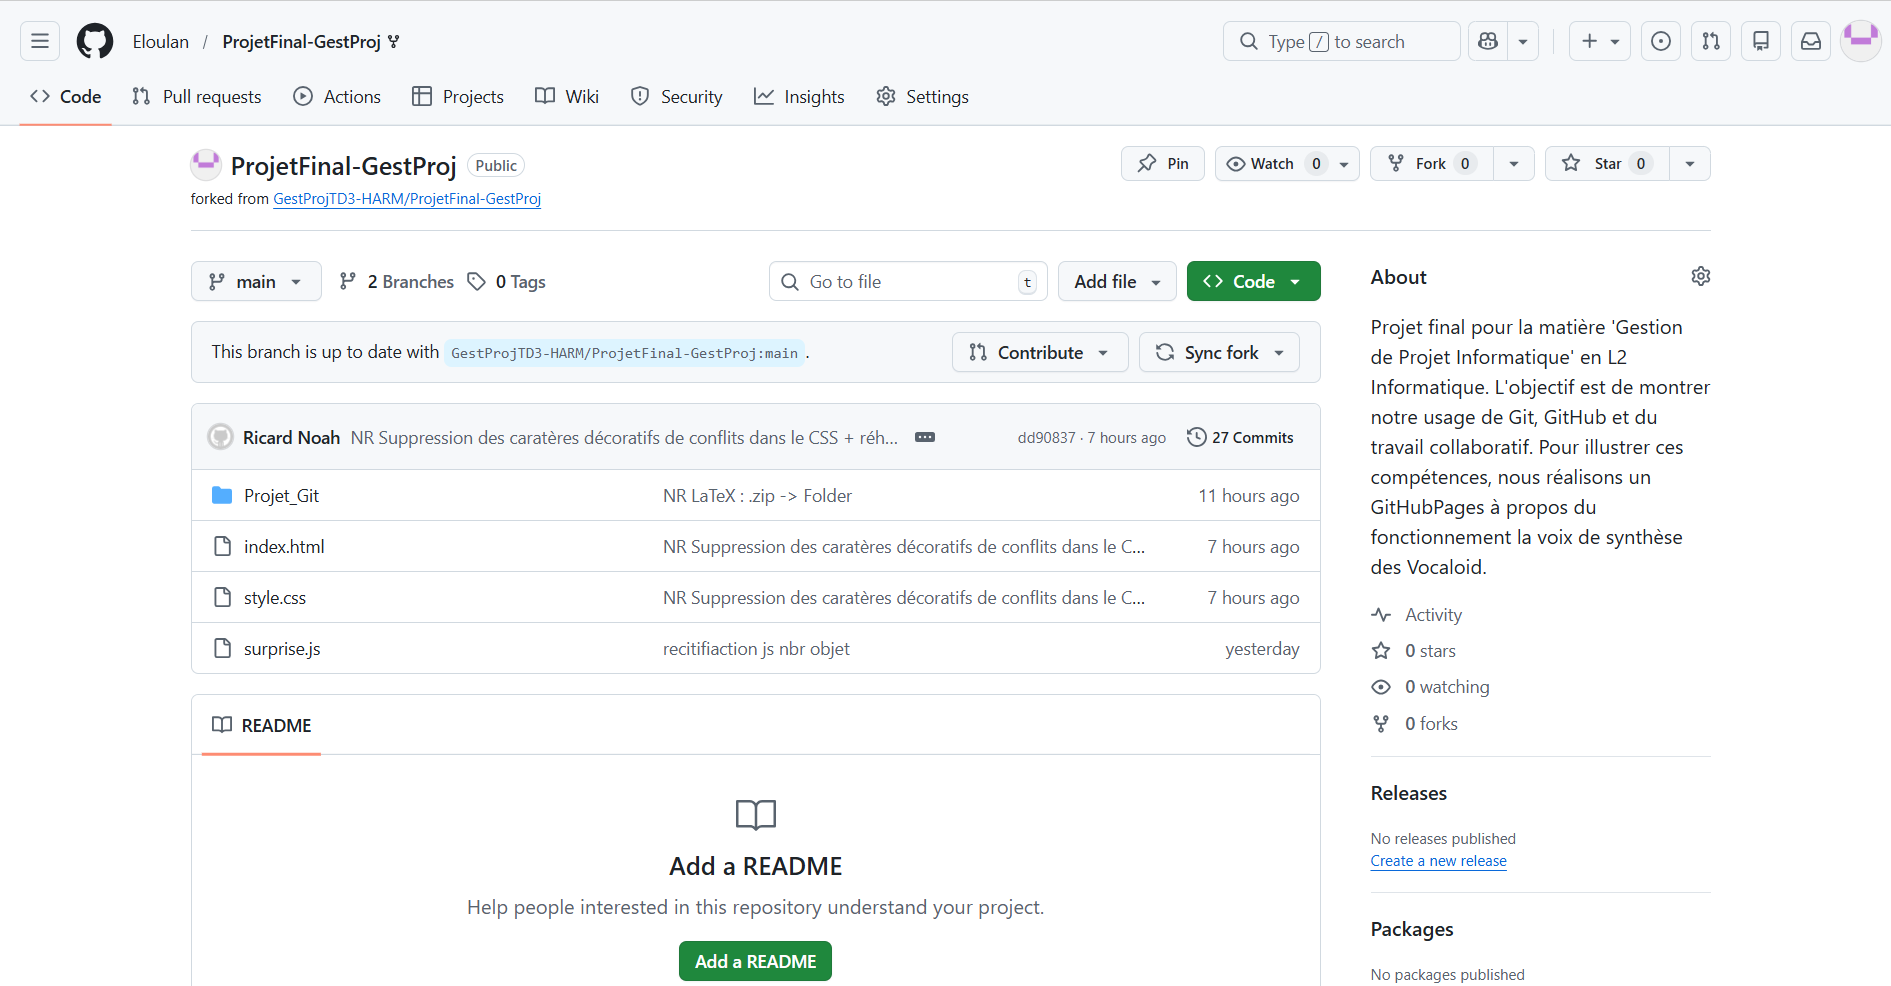
\includegraphics[width=0.5\textwidth]{Repository.png}
    \caption{Le dépôt du mini-projet}
\end{figure}
Grâce à ce dépôt l'équipe peut facilement échanger leurs ajouts de façon pratique et immédiate,... %Restitution du cours
\\Les étapes suivantes seront plus orientées vers la construction d'un environnements GitHub profitant d'un maximum de ces fonctions


\section*{\color{Green}[A3] Intégration des contributions}
Les premiers commits, n'ayant pas encore à ce moment associés tous le monde en collaborateurs, ont un nom différent lors des commits (\ref{fig:first-commits}). %Desolé Noah enfaite c'est moi qui commit avec DES ordis diffèrents (celui du cours, celui de chez moi, une session pour chaque ordi de la salle info)

Chaque membres peut push de son côtés et après verifications de la part des autres, être affectées au projet finale.
\begin{figure}[ht]
    \centering
    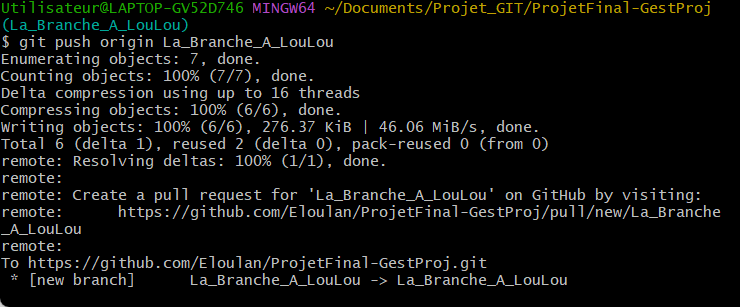
\includegraphics[width=0.5\linewidth]{PushCommand.png}
    \includegraphics[width=0.5\linewidth]{First-commits.png}
    \caption{Capture d'écran d'un push vers le dépôt et des premiers commits push vers le projet principale}
    \label{fig:first-commits}
\end{figure}

\section*{\color{BurntOrange}[B1] Gestion par branches}
Je m'apprête à créer une branche pour cette version car les marges du LaTeX m'ont été proposée à 1.5cm mais je pense que 2.5cm pourrait être mieux. Pourquoi pas un entre deux, le LaTeX devra être restructuré dans le cas d'un changement de marge avant qu'un 'merge' soit fait avec la branche principale.
\begin{figure}[ht]
    \centering
    
\includegraphics[width=0.7\linewidth]{BranchCommand.png}
    
\includegraphics[width=0.7\linewidth]{CheckoutBranchCommand.png}
    \caption{Création d'une branche pour les changements du LaTeX}
    \label{fig:Branch_latex}
\end{figure}

\section*{\color{BurntOrange}[B2] Intégration de version et tag}

\section*{\color{BurntOrange}[B3] Gestion des propositions de contributions}

\section*{\color{BurntOrange}[B4] Intégration de site web}

Lien du GitHubPages : \url{https://gestprojtd3-harm.github.io/ProjetFinal-GestProj/}

\section*{\color{BrickRed}[C1] Répartition de tâches et milestone}

\section*{\color{BrickRed}[C2] Intégration continue}

\section*{\color{BrickRed}[C3] Gestion de submodule}

\section*{\color{BrickRed}[C4] Gestion par l'outil \textit{Projet} de \textit{GitHub}}

\end{document}